\documentclass[tikz,border=3.14mm]{standalone}
\usepackage{tikz}
\begin{document}

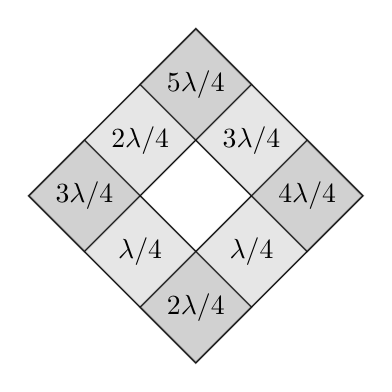
\begin{tikzpicture}[rotate=45]

    % Основной квадрат (повернут на 45 градусов)
    \draw (0,0) rectangle (3,3);

    % Разделение на 3x3 квадратов
    \foreach \x in {1,2} { \draw (\x,0) -- (\x,3); \draw (0,\x) -- (3,\x); }

    % Добавляем прямоугольники 1x3 по сторонам
    \draw[fill=gray!100, opacity=0.2, thick] (0,0) rectangle (1,3); 
    \draw[fill=gray!100, opacity=0.2, thick] (0,0) rectangle (3,1); 
    \draw[fill=gray!100, opacity=0.2, thick] (2,0) rectangle (3,3); 
    \draw[fill=gray!100, opacity=0.2, thick] (0,3) rectangle (3,2); 

    % Добавляем текст "Text" параллельно сторонам
    \node[rotate=0] at (0.5,1.5) {$\lambda/4$}; %левый нижний 
    \node[rotate=0] at (1.5,0.5) {$\lambda/4$}; %правый нижний
    \node[rotate=0] at (2.5,1.5) {$3\lambda/4$}; %правый верхний
    \node[rotate=0] at (1.5,2.5) {$2\lambda/4$}; % левый верхний 

    \node[rotate=0] at (0.5,0.5) {$2\lambda/4$};
    \node[rotate=0] at (2.5,2.5) {$5\lambda/4$};
    \node[rotate=0] at (2.5,0.5) {$4\lambda/4$};
    \node[rotate=0] at (0.5,2.5) {$3\lambda/4$};
\end{tikzpicture}

\end{document}